\begin{pa} \label{PA:7.2}
Let's consider the initial value problem 
$$
\frac{dy}{dt} = t - 2, \ \ y(0) = 1.
$$

\ba
\item Use the differential equation to find the slope of the tangent
  line to the solution $y(t)$ at $t=0$.  Then use the initial value to
  find the equation of the tangent line at $t=0$.  Sketch this tangent
  line over the interval $-0.25\leq t\leq0.25$ on the axes provided.

  \begin{center}
    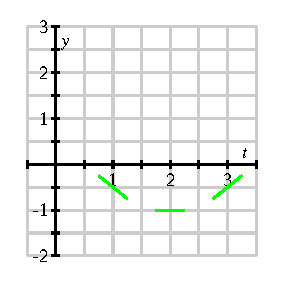
\includegraphics{figures/7_2_PA_tangents.eps}
  \end{center}

\item Also shown in the given figure are the tangent lines to the solution $y(t)$ at
  the points $t=1, 2,$ and $3$ (we will see how to find these later).
  Use the graph to measure the slope of each tangent line  
  and verify that each agrees with the value specified by the differential
  equation.  

\item Using these tangent lines as a guide, sketch a graph of the
  solution $y(t)$ over the interval $0\leq t\leq 3$ so that the lines
  are tangent to the graph of $y(t)$.

\item Use the Fundamental Theorem of Calculus to find $y(t)$, the
  solution to this initial value problem.

\item Graph the solution you found in (d) on the axes provided, and compare it to the sketch
  you made using the tangent lines.

\ea
\end{pa} 
\afterpa
